\documentclass{article}
\usepackage[utf8]{inputenc}
\usepackage{xcolor}
\usepackage{graphicx}
\usepackage{float}
\usepackage{minted}
\usepackage{circuitikz}
\usepackage{tikz}
\usetikzlibrary{shapes, arrows, calc, positioning, circuits.logic.US, circuits.logic.IEC}
\usepackage{geometry}
\geometry{a4paper, margin=1in}
\usepackage{hyperref}
\usemintedstyle{trac}

\title{Laboratory Exercise 6 \\ Latches, Flip-flops, and Registers}
\date{}

\begin{document}

\maketitle

The purpose of this exercise is to investigate latches, flip-flops, and registers.

\section*{Part I}

Intel FPGAs include flip-flops that are available for implementing a user's circuit. We will show how to make use of these flip-flops in Part IV of this exercise. But first we will show how storage elements can be created in an FPGA without using its dedicated flip-flops.

Figure 1 depicts a gated RS latch circuit. A style of VHDL code that uses logic expressions to describe this circuit is given in Figure 2. If this latch is implemented in an FPGA that has 4-input lookup tables (LUTs), then only one lookup table is needed, as shown in Figure 3a.

\begin{figure}[htbp]
    \centering
    % Placeholder for Figure 1: Gated RS Latch
    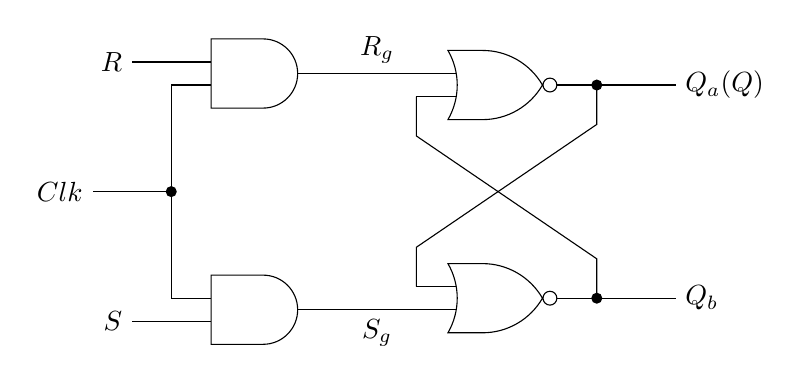
\begin{tikzpicture}[circuit logic US, huge circuit symbols]
    % Gates
    \node[and gate, inputs={nn}] (A1) at (0, 1.5) {};
    \node[and gate, inputs={nn}] (A2) at (0, -1.5) {};
    \node[nor gate, inputs={nn}, anchor=input 1] (O1) at ($(A1.output) + (2, 0)$) {};
    \node[nor gate, inputs={nn}, anchor=input 2] (O2) at ($(A2.output) + (2, 0)$) {};

    % Labels for internal signals (removed explicit nodes, added to paths below)

    % Inputs
    \draw (A1.input 1) -- ++(-1,0) node[left] {$R$};
    \draw (A2.input 2) -- ++(-1,0) node[left] {$S$};
    
    % Clock connection
    \draw (A1.input 2) -- ++(-0.5,0) coordinate (clk_top);
    \draw (A2.input 1) -- ++(-0.5,0) coordinate (clk_bot);
    \draw (clk_top) -- (clk_bot);
    \draw ($(clk_top)!0.5!(clk_bot)$) coordinate (clk_mid);
    \fill (clk_mid) circle (2pt);
    \draw (clk_mid) -- ++(-1,0) node[left] {$Clk$};

    % Connections to NOR latch with centered labels
    \draw (A1.output) -- node[above] {$R_g$} (O1.input 1);
    \draw (A2.output) -- node[below] {$S_g$} (O2.input 2);

    % Latch feedback with crossed lines
    \draw (O1.input 2) -- ++(-0.5, 0) coordinate (O1_fb_in);
    \draw (O2.input 1) -- ++(-0.5, 0) coordinate (O2_fb_in);

    % Feedback paths
    \draw (O1.output) -- ++(0.5,0) coordinate (Qa_out);
    \fill (Qa_out) circle (2pt);
    
    \draw (O2.output) -- ++(0.5,0) coordinate (Qb_out);
    \fill (Qb_out) circle (2pt);

    % Cross routing
    % Define intermediate points to avoid syntax errors
    \path (O2_fb_in) ++(-0,0.5) coordinate (O2_cross_x);
    \path (O1_fb_in) ++(-0,-0.5) coordinate (O1_cross_x);

    % Qa (Top) -> Bottom Input (O2)
    \draw (Qa_out) -- ++(0,-0.5) coordinate (Qa_drop) -- (O2_cross_x) -- (O2_fb_in);
    
    % Qb (Bottom) -> Top Input (O1)
    \draw (Qb_out) -- ++(0,0.5) coordinate (Qb_drop) -- (O1_cross_x) -- (O1_fb_in);

    % Outputs
    \draw (Qa_out) -- ++(1,0) node[right] {$Q_a (Q)$};
    \draw (Qb_out) -- ++(1,0) node[right] {$Q_b$};

\end{tikzpicture}

    \caption{A gated RS latch circuit.}
    \label{fig:gated_rs_latch}
\end{figure}

\begin{figure}[htbp]
    \centering
    \begin{minted}[frame=single, fontsize=\small, linenos]{vhdl}
LIBRARY ieee;
USE ieee.std_logic_1164.all;

ENTITY part1 IS
    PORT ( Clk, R, S : IN STD_LOGIC;
           Q : OUT STD_LOGIC);
END part1;

ARCHITECTURE Structural OF part1 IS
    SIGNAL R_g, S_g, Qa, Qb : STD_LOGIC ;
    ATTRIBUTE KEEP : BOOLEAN;
    ATTRIBUTE KEEP OF R_g, S_g, Qa, Qb : SIGNAL IS TRUE;
BEGIN
    R_g <= R AND Clk;
    S_g <= S AND Clk;
    Qa <= NOT (R_g OR Qb);
    Qb <= NOT (S_g OR Qa);
    Q <= Qa;
END Structural;
    \end{minted}
    \caption{Specifying the RS latch by using logic expressions.}
    \label{fig:vhdl_rs_latch}
\end{figure}

Although the latch can be correctly realized in one 4-input LUT, this implementation does not allow its internal signals, such as $R\_g$ and $S\_g$, to be observed, because they are not provided as outputs from the LUT. To preserve these internal signals in the implemented circuit, it is necessary to include a compiler directive in the code. In Figure 2 the directive KEEP is included by using a VHDL ATTRIBUTE statement to instruct the Quartus compiler to use separate logic elements for each of the signals $R\_g$, $S\_g$, $Qa$, and $Qb$. Compiling the code produces the circuit with four 4-LUTs depicted in Figure 3b.

\begin{figure}[htbp]
    \centering
    % Placeholder for Figure 3
    \caption{Implementation of the RS latch from Figure 1.}
    \label{fig:rs_latch_impl}
\end{figure}

Create a Quartus project for the RS latch circuit as follows:
\begin{enumerate}
    \item Create a new Quartus project for your DE0-CV board.
    \item \textbf{First, implement the circuit using Schematic Design.} Draw the circuit using the Block Editor and appropriate logic gates.
    \item Compile the schematic design and perform a functional simulation to verify its correctness. Ensure the behavior matches the expected RS latch operation.
    \item \textbf{Next, implement the circuit using Structural VHDL Design.}
    \item Generate a VHDL file with the code in Figure 2 and include it in the project.
    \item Compile the code. Use the Quartus RTL Viewer tool to examine the gate-level circuit produced from the code, and use the Technology Map Viewer tool to verify that the latch is implemented as shown in Figure 3b.
    \item Simulate the behavior of your VHDL code by using the simulation feature provided in the Quartus software. First, create a vector waveform file (*.vwf) using the Quartus software to specify the inputs and outputs of your circuit. Then, use the commands available in the Quartus Simulation Waveform Editor tool to run a simulation of the circuit.
\end{enumerate}

\begin{figure}[htbp]
    \centering
    % Placeholder for Figure 4
    \caption{Simulation waveforms for the RS latch.}
    \label{fig:sim_rs_latch}
\end{figure}

\section*{Part II}

Figure 5 shows the circuit for a gated D latch.

\begin{figure}[htbp]
    \centering
    % Placeholder for Figure 5: Gated D Latch
    \input{tex/lab6p2_gated_d_latch.tex}
    \caption{Circuit for a gated D latch.}
    \label{fig:gated_d_latch}
\end{figure}

Perform the following steps:
\begin{enumerate}
    \item Create a new Quartus project.
    \item \textbf{First, implement the circuit using Schematic Design.} Draw the circuit using the Block Editor.
    \item Compile the schematic design and perform a functional simulation to verify its correctness.
    \item \textbf{Next, implement the circuit using Structural VHDL Design.}
    \item Modify the VHDL code from Part I to implement the gated D latch. Use the KEEP directive to ensure that separate logic elements are used to implement the signals R, S\_g, R\_g, Qa, and Qb.
    \item Compile your project and then use the Technology Map Viewer tool to examine the implemented circuit.
    \item Verify that the latch works properly for all input conditions by using functional simulation. Examine the timing characteristics of the circuit by using timing simulation.
    \item Create a new Quartus project which will be used for implementation of the gated D latch on your DE0-CV board. This project should consist of a top-level module that contains the appropriate input and output ports (pins) for your board. Instantiate your latch in this top-level module. Use switch SW0 to drive the D input of the latch, and use SW1 as the Clk input. Connect the Q output to LEDR0.
    \item Include the required pin assignments and then compile your project and download the compiled circuit onto your DE0-CV board.
    \item Test the functionality of your circuit by toggling the D and Clk switches and observing the Q output.
\end{enumerate}

\section*{Part III}

Figure 6 shows the circuit for a master-slave D flip-flop.

\begin{figure}[htbp]
    \centering
    % Placeholder for Figure 6: Master-Slave D Flip-Flop
    \begin{circuitikz}
    \ctikzset{logic ports=ieee}
    \ctikzset{flipflops/scale=1}
    % Define standard D Latch style
    \tikzset{d-latch/.style={flipflop, flipflop def={
        t1=D, t3=C, t4={\ctikztextnot{Q}}, t6=Q
    }}}
    % Define Negated Enable D Latch style (for Slave)
    \tikzset{d-latch-n/.style={flipflop, flipflop def={
        t1=D, t3=C, t4={\ctikztextnot{Q}}, t6=Q
    }}}

    % Master Latch (Active High Enable)
    \node[d-latch] (Master) at (0,0) {Master};
    
    % Slave Latch (Active Low Enable via Bubble)
    \node[d-latch-n] (Slave) at (5,0) {Slave};
    
    % Inputs
    % Input D
    \draw (Master.pin 1) -- ++(-1.5, 0) coordinate (D_in) node[left] {D};
    
    % Clock Input common point
    % Align Clock horizontal start point with D node x-coordinate
    \coordinate (Clk_pin) at (Master.pin 3);
    
    % Clock Source
    \coordinate (Clk_in_Node) at ($(D_in) + (0,-2.5)$); % Lower down
    \draw (Clk_in_Node) node[left] {Clk} -- ++(1.5,0) coordinate (clk_main_split);
    \fill (clk_main_split) circle (2pt);
    
    % Connect Clock to Master Enable (Active High)
    % Route: Split -> Right -> Up -> Master Pin 3
    \draw (clk_main_split) -| (Master.pin 3);
    
    % Connect Clock to Slave Enable (Active Low)
    % Route: Split -> Right -> Right -> Up -> Slave Pin 3
    \draw (clk_main_split) -- ++(3,0) node[not port,anchor=in,scale=0.5] (not_port) {};
    \draw (not_port.out) -| (Slave.pin 3);
    
    % Logic:
    % Clk=1: Master En (Transp), Slave Dis (Hold).
    % Clk=0: Master Dis (Hold), Slave En (Transp).
    % Negative Edge Triggered.

    % Wiring Master Q -> Slave D
    \draw (Master.pin 6) -- (Slave.pin 1);
    
    % Outputs
    \draw (Slave.pin 6) -- ++(1, 0) node[right] {$Q$};
    \draw (Slave.pin 4) -- ++(1, 0) node[right] {$\bar{Q}$};

\end{circuitikz}

    \caption{Circuit for a master-slave D flip-flop.}
    \label{fig:master_slave_ff}
\end{figure}

Perform the following:
\begin{enumerate}
    \item Create a new Quartus project.
    \item \textbf{First, implement the circuit using Schematic Design.} Create a symbol for the Gated D latch from Part II and use it to build the circuit.
    \item Compile the schematic design and perform a functional simulation to verify its correctness.
    \item \textbf{Next, implement the circuit using Structural VHDL Design.}
    \item Create a VHDL entity/component for the gated D latch from Part II. Then, write a top-level VHDL file that instantiates two copies of this component to implement the master-slave flip-flop.
    \item Include in your project the appropriate input and output ports for your DE0-CV board. Use switch SW0 to drive the D input of the flip-flop, and use SW1 as the Clock input. Connect the Q output to LEDR0.
    \item Include the required pin assignments and then compile your project.
    \item Use the Technology Viewer to examine the D flip-flop circuit, and use simulation to verify its correct operation.
    \item Download the circuit onto your DE0-CV board and test its functionality by toggling the D and Clock switches and observing the Q output.
\end{enumerate}

\section*{Part IV}

Figure 7 shows a circuit with three different storage elements: a gated D latch, a positive-edge triggered D flip-flop, and a negative-edge triggered D flip-flop.

\begin{figure}[htbp]
    \centering
    % Placeholder for Figure 7: Three storage elements
    \begin{circuitikz}
    \ctikzset{logic ports=ieee}
    \ctikzset{flipflops/scale=1}

    % Define Styles
    % Latch: Transparent high (no clock wedge)
    \tikzset{latch/.style={flipflop, flipflop def={t1=D, t3=Clk, t6=Q}}} 
    % Pos-Edge FF: Standard D FF with clock wedge
    \tikzset{pos-ff/.style={flipflop D, flipflop def={t6=Q}}}
    % Neg-Edge FF: Standard D FF with clock wedge and negation
    \tikzset{neg-ff/.style={flipflop D, flipflop def={t6=Q, n3=1}}}

    % Nodes
    % 1. Gated D Latch
    \node[latch] (latch) at (0, 0) {};
    \node[above] at (latch.north) {Gated D Latch};

    % 2. Pos-Edge D FF
    \node[pos-ff] (pos_ff) at (0, -3.5) {};
    \node[above] at (pos_ff.north) {Pos-Edge D FF};

    % 3. Neg-Edge D FF
    \node[neg-ff] (neg_ff) at (0, -7) {};
    \node[above] at (neg_ff.north) {Neg-Edge D FF};

    % Inputs aligned to latch
    % D connected to Latch Pin 1 (D)
    % Clock connected to Latch Pin 3 (Clk)
    \coordinate (D_pin) at (latch.pin 1);
    \coordinate (Clk_pin) at (latch.pin 3);
    
    \draw (D_pin) -- ++(-3, 0) node[left] (D_in) {D};
    \draw (Clk_pin) -- ++(-3, 0) node[left] (Clk_in) {Clock};

    % Bus Lines
    % Vertical bus for D
    \coordinate (D_bus_top) at ($(D_in.east) + (0.5, 0)$);
    \draw (D_bus_top) |- (pos_ff.pin 1);
    \draw (D_bus_top) |- (neg_ff.pin 1);
    \draw (D_bus_top) -- (D_pin); % Connect to latch D
    \fill[black] (D_bus_top) circle (2pt);
    \fill[black] (D_bus_top |- pos_ff.pin 1) circle (2pt);

    % Vertical bus for Clock
    \coordinate (Clk_bus_top) at ($(Clk_in.east) + (1.0, 0)$);
    \draw (Clk_bus_top) |- (pos_ff.pin 3);
    \draw (Clk_bus_top) |- (neg_ff.pin 3);
    \draw (Clk_bus_top) -- (Clk_pin); % Connect to latch Clk
    \fill[black] (Clk_bus_top) circle (2pt);
    \fill[black] (Clk_bus_top |- pos_ff.pin 3) circle (2pt);

    % Outputs
    \draw (latch.pin 6) -- ++(1, 0) node[right] {$Q_a$};
    \draw (pos_ff.pin 6) -- ++(1, 0) node[right] {$Q_b$};
    \draw (neg_ff.pin 6) -- ++(1, 0) node[right] {$Q_c$};

\end{circuitikz}

    \caption{Circuit for Part IV.}
    \label{fig:three_storage}
\end{figure}

\begin{figure}[htbp]
    \centering
    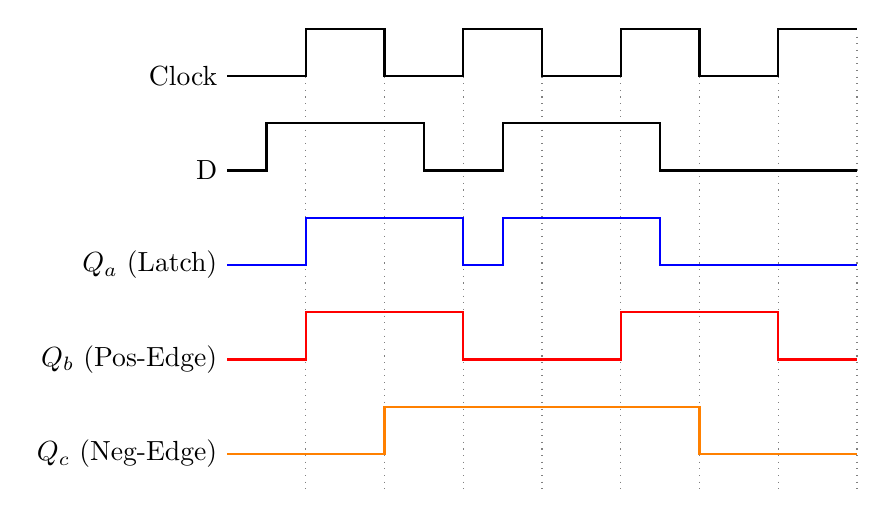
\begin{tikzpicture}
    % Define coordinates
    \def\tick{0.2}
    \def\h{0.6} % Height of logic high
    \def\sep{-1.2} % Separation between signals

    % Labels
    \node[anchor=east] at (0, 0) {Clock};
    \node[anchor=east] at (0, \sep) {D};
    \node[anchor=east] at (0, 2*\sep) {$Q_a$ (Latch)};
    \node[anchor=east] at (0, 3*\sep) {$Q_b$ (Pos-Edge)};
    \node[anchor=east] at (0, 4*\sep) {$Q_c$ (Neg-Edge)};

    % Draw Axes/Grid lines
    \foreach \x in {1,2,...,8} {
        \draw[dotted, gray] (\x, 0.5) -- (\x, 4*\sep - 0.5);
    }

    % Clock Signal (Period = 2 units)
    % 0-1 Low, 1-2 High...
    \draw[thick] (0,0) -- (1,0) -- (1,\h) -- (2,\h) -- (2,0) -- (3,0) -- (3,\h) -- (4,\h) -- (4,0) -- (5,0) -- (5,\h) -- (6,\h) -- (6,0) -- (7,0) -- (7,\h) -- (8,\h);

    % D Input (Arbitrary)
    % 0-0.5: 0
    % 0.5-2.5: 1
    % 2.5-3.5: 0
    % 3.5-5.5: 1
    % 5.5-8.0: 0
    \draw[thick] (0, \sep) -- (0.5, \sep) -- (0.5, \sep+\h) -- (2.5, \sep+\h) -- (2.5, \sep) -- (3.5, \sep) -- (3.5, \sep+\h) -- (5.5, \sep+\h) -- (5.5, \sep) -- (8, \sep);

    % Qa (Gated D Latch) - Transparent when Clk=1
    \draw[thick, blue] (0, 2*\sep) 
        -- (1, 2*\sep)       % Hold 0
        -- (1, 2*\sep+\h)    % @1.0 Clk->1, D=1 -> 1
        -- (3, 2*\sep+\h)    % Hold 1 until 3.0
        -- (3, 2*\sep)       % @3.0 become 0
        -- (3.5, 2*\sep)     % Follow 0
        -- (3.5, 2*\sep+\h)  % @3.5 D->1, Clk=1 -> Follow 1
        -- (5.5, 2*\sep+\h)  % Hold/Follow 1
        -- (5.5, 2*\sep)     % @5.5 Follow 0
        -- (8, 2*\sep);      % 0

    % Qb (Pos-Edge D FF) - Sample D at Rising Edge (1, 3, 5, 7)
    \draw[thick, red] (0, 3*\sep) 
        -- (1, 3*\sep)    % Init 0
        -- (1, 3*\sep+\h) % @1 D=1 -> 1
        -- (3, 3*\sep+\h) % Hold
        -- (3, 3*\sep)    % @3 D=0 -> 0
        -- (5, 3*\sep)    % Hold
        -- (5, 3*\sep+\h) % @5 D=1 -> 1
        -- (7, 3*\sep+\h) % Hold
        -- (7, 3*\sep)    % @7 D=0 -> 0
        -- (8, 3*\sep);

    % Qc (Neg-Edge D FF) - Sample D at Falling Edge (2, 4, 6)
    \draw[thick, orange] (0, 4*\sep) 
        -- (2, 4*\sep)    % Init 0
        -- (2, 4*\sep+\h) % @2 D=1 -> 1
        -- (6, 4*\sep+\h) % Hold
        -- (6, 4*\sep)    % @6 D=0 -> 0
        -- (8, 4*\sep);

\end{tikzpicture}

    \caption{Waveforms for Part IV.}
    \label{fig:three_storage_timing}
\end{figure}

Implement and simulate this circuit using the Quartus software as follows:
\begin{enumerate}
    \item Create a new Quartus project.
    \item \textbf{First, implement the circuit using Schematic Design.} Draw the circuit using the Block Editor.
    \item Compile the schematic design and perform a functional simulation to verify its correctness.
    \item \textbf{Next, implement the circuit using Structural VHDL Design.}
    \item Write a VHDL file that instantiates the three storage elements. For this part you should no longer use the KEEP directive.
    \item Compile your code and use the Technology Map Viewer to examine the implemented circuit. Verify that the latch uses one lookup table and that the flip-flops are implemented using the flip-flops provided in the target FPGA.
    \item Create a Vector Waveform File (.vwf) that specifies the inputs and outputs of the circuit. Draw the inputs D and Clock as indicated in Figure 7. Use functional simulation to obtain the three output signals. Observe the different behavior of the three storage elements.
\end{enumerate}

\section*{Part V}

We wish to display the hexadecimal value of an 8-bit number A on the two 7-segment displays HEX3-2. We also wish to display the hex value of an 8-bit number B on the two 7-segment displays HEX1-0. The values of A and B are inputs to the circuit which are provided by means of switches SW7-0. To input the values of A and B, first set the switches to the desired value of A, store these switch values in a register, and then change the switches to the desired value of B. Finally, use an adder to generate the arithmetic sum S = A + B, and display this sum on the 7-segment displays HEX5-4. Show the carry-out produced by the adder on LEDR(0).

\begin{enumerate}
    \item Create a new Quartus project which will be used to implement the desired circuit on your DE0-CV board.
    \item \textbf{Implement the circuit using Structural VHDL Design.} Write a VHDL file that provides the necessary functionality. Use KEY0 as an active-low asynchronous reset, and use KEY1 as a clock input.
    \item Include the necessary pin assignments for the pushbutton switches and 7-segment displays, and then compile the circuit.
    \item Download the circuit onto your DE0-CV board and test its functionality by toggling the switches and observing the output displays.
\end{enumerate}

\vspace{1cm}
\noindent \textbf{Updated By:} R. Sutthaweekul \\
\textbf{Release Date:} 2026-01-01

\end{document}
